%%%%%%%%%%%%%%%%%%%%%%%%%%%%%%%%%%%%%%%%%%%%%%%%%%%%%%%%%%%%%%%%%%%%%
% In English:
%    This is a Latex template for São Paulo Research Foudation (FAPESP)
%         reports (annual or final).
%    This is the modified version of the original Latex template from
%         following website.
%    Original Source: http://www.howtotex.com
%    For information about FAPESP, check http://www.fapesp.br/en
%    This template targets mainly on reports in Portuguese language.
%    New additions and changes in the latest version:
%        - Added the possibility of including multiple members in the
%          research team, with the commands \memberA{Name of Member A}
%          \memberB{Name of Member B} \memberC{Name of Member C} etc.
%        - Included commands to define project modality and the research
%          agency (if you want to use the same model for other research
%          agencies such as CAPES, CNPq etc).
%
% In Portuguese:
%    Este é um modelo Latex para relatórios (anual ou final) da Fundação
%         de Amparo à pesquisa do Estado de São Paulo (FAPESP).
%    Esta é uma versão modificada do modelo Latex do site supra mencionado.
%    Para informações sobre a FAPESP, verifique http://www.fapesp.br
%    Esse modelo foca principalmente nos relatórios escritos em Português.
%    Novas adições e alterações na última versão:
%       - Foi adicionada a possibilidade de incluir vários membros no
%         grupo de pesquisas, com os comandos \membroA{Nome do Membro A}
%         \membroB{} \membroC{} etc.
%       - Foram incluídos comandos para definir modalidade de projeto e
%         agência de fomento (caso queira utilizar o mesmo modelo para
%         outras agências, CAPES, CNPq etc).
%
% Author/Autor: André Leon Sampaio Gradvohl, Dr.
% Email:        andre.gradvohl@gmail.com
% Lattes CV:    http://lattes.cnpq.br/9343261628675642
% GitHub: http://gradvohl.github.io/
%
% Last update/Última versão: 19/Feb/2018
%
%%%%%%%%%%%%%%%%%%%%%%%%%%%%%%%%%%%%%%%%%%%%%%%%%%%%%%%%%%%%%%%%%%%%%%
\documentclass[12pt]{report}
\usepackage[a4paper]{geometry}
\usepackage[utf8]{inputenc}
\usepackage[english]{babel}
\usepackage[myheadings]{fullpage}
\usepackage[T1]{fontenc}
\usepackage{fancyhdr}
\usepackage{setspace}
\usepackage{sectsty}
\usepackage{url}

%%% iniciar capitulo na mesma pagina (Mateus) %%%
\usepackage{etoolbox}
\makeatletter %inicio da modificacao (iniciar capitulo na msma pag)
\patchcmd{\chapter}{\if@openright\cleardoublepage\else\clearpage\fi}{}{}{}
\makeatother %fim da modificacao
%%% iniciar capitulo na mesma pagina (Mateus) %%%

%%------
%% Comandos gerais
%% Observação: o arquivo "comandos.tex" tem que estar presente.
%%------
%%%%%%%%%%%%%%%%%%%%%%%%%%%%%%%%%%%%%%%%%%%%%%%%%%%%%%%%%%%%%%%%%%%%%
% In English:
%    This is a list of commands specification for FAPESP reports.
%
% In Portuguese:
%    Esta é uma lista de especificação de comandos para relatórios
% da Fundação de Amparo à pesquisa do Estado de São Paulo (FAPESP).
%
% Author/Autor: André Leon Sampaio Gradvohl, Dr.
% Email:        andre.gradvohl@gmail.com
% Lattes CV:    http://lattes.cnpq.br/9343261628675642
%
% Last update/Última versão: 11/Sep/2016
%%%%%%%%%%%%%%%%%%%%%%%%%%%%%%%%%%%%%%%%%%%%%%%%%%%%%%%%%%%%%%%%%%%%%%

\newcommand{\HRule}[1]{\rule{\linewidth}{#1}}
\setcounter{tocdepth}{3}
\setcounter{secnumdepth}{3}

\newcommand{\titulo}[1]{\def\meuTitulo{#1}}
\newcommand{\tituloIngles}[1]{\def\meuTituloIngles{#1}}
\newcommand{\numProjeto}[1]{\def\numFAP{#1}}
\newcommand{\tipoRelatorio}[1]{\def\tipoRelat{#1 }} %o espaço depois do #1 é importante
\newcommand{\modalidadeProjeto}[1]{\def\modProjeto{#1}}
\newcommand{\agFomento}[2]{\def\agFom{#1} \def\siglaAgFom{#2}} %extenso Sigla
\newcommand{\autor}[1]{\def\nomeAutor{#1}}
\newcommand{\cidade}[1]{\def\nomeCidade{#1}}
\newcommand{\universidade}[1]{\def\nomeUniversidade{#1}}
\newcommand{\faculdade}[1]{\def\nomeFaculdade{#1}}
\newcommand{\periodoVigencia}[1]{\def\periodVig{#1}}
\newcommand{\periodoRelatorio}[1]{\def\periodRelat{#1}}
\newcommand{\orientador}[1]{\def\nomeOrientador{#1}}

\newcommand\namegroup[3]{%
   \begin{minipage}[t]{0.4\textwidth}
   \hspace{0.6cm}
   \begin{tikzpicture}
   \node[anchor=south east,inner sep = 0](signF){\includegraphics[width=#3]{#2}};
   \end{tikzpicture}
   \vspace*{0.1cm}  % leave some space above the horizontal line
   \hrule
   \vspace{1mm} % just a bit more whitespace below the line
   \centering
   \begin{tabular}[t]{c}
   #1
   \end{tabular}
   \end{minipage}}

\author{}
\date{}

%Definição de membros da equipe de pesquisas
\newcommand{\membroA}[1]{\def\nomeMembroA{#1}}
\newcommand{\membroB}[1]{\def\nomeMembroB{#1}}
\newcommand{\membroC}[1]{\def\nomeMembroC{#1}}
\newcommand{\membroD}[1]{\def\nomeMembroD{#1}}
\newcommand{\membroE}[1]{\def\nomeMembroE{#1}}
\newcommand{\membroF}[1]{\def\nomeMembroF{#1}}

\newcommand{\Figure}[1]{Figura~\ref{fig:#1}}
\newcommand{\Table}[1] {Tabela~\ref{#1}}
\newcommand{\Equation}[1] {Equa\c{c}\~ao~\ref{#1}}
\newcommand{\addFigure}[3] { %Parametros scale, fig_name, caption
    \begin{figure}[!hbt]
      \centering
      \includegraphics[scale=#1]{figures/}
      \caption{#3}\label{fig:#2}
    \end{figure}
}

\newcommand{\geraTitulo}{
\clearpage
\begin{titlepage}
  \begin{center}
      \vspace*{-3cm}
       { \setstretch{.5}
         \textsc{\nomeUniversidade} \\
         \HRule{.2pt}\\
         \textsc{\nomeFaculdade}
       }

       \vspace{5.5cm}

       \Large \textbf{\textsc{\meuTitulo}}
 	  \HRule{1.5pt} \\ [0.5cm]
       \linespread{1}
       \large Final report on the activities
       %\ifdefined\tipoRelat
       %     \tipoRelat
       %\fi
       of the
       \ifdefined\modProjeto
           \modProjeto
       \fi
       ~project supported by the \agFom. \\
   	   \HRule{1.5pt} \\ [0.5cm]

       \ifdefined\numFAP
          Grant \texttt{\#\numFAP}, \siglaAgFom
          \\ [0.5cm]
       \fi
        Author: \nomeAutor \\
        Advisor: \nomeOrientador \\[5.cm]

        % aqui começa a adicao das linhas de assinatura
        %Aluno: \tikz\draw [thick,solid] (0,0) -- (6,0); \\[.5cm]
        %Orientador: \tikz\draw [thick,solid] (0,0) -- (5.5,0);


        %% Assinatura assinatura ASSINATURA
        %\namegroup{Researcher}{example-image-a}
        \namegroup{Researcher}{fig/assinatura-mateus.png}{5cm}
        \hspace{1.5cm}
        \namegroup{Advisor}{fig/placeholder.png}{1cm}

        %\begin{minipage}[t]{0.4\textwidth}
        %\vspace*{1.5cm}
        %\hrule
        %\vspace{1mm}
        %\centering
        %\begin{tabular}[t]{c}
        %Aluno
        %\end{tabular}
        %\hspace{1.5cm}
        %\begin{minipage}[t]{0.4\textwidth}
        %\vspace*{1.5cm}
        %\hrule
        %\vspace{1mm}
        %\centering
        %\begin{tabular}[t]{c}
        %Aluno
        %\end{tabular}
        %\end{minipage}
        %%\hfill

        \vfill

        {\normalsize  \nomeCidade, \today}
 \end{center}
 \end{titlepage}
}

\usepackage{titlesec}
\titleformat{\chapter}{\normalfont\LARGE\bfseries}{\thechapter}{1em}{}
\titlespacing*{\chapter}{0pt}{3.5ex plus 1ex minus .2ex}{2.3ex plus .2ex}

%----------------------------------------------------------------------
% Cabeçalho e rodapé
%----------------------------------------------------------------------
\pagestyle{fancy}
\fancyhf{} % Limpa todos os campos de header and footer fields
\renewcommand{\headrulewidth}{0pt}
\fancyfoot[R]{\thepage}

\addto\captions{\renewcommand{\contentsname}{Summary}}
\addto\captions{\renewcommand{\bibname}{Bibliography}}

%------
% Resumo e Abstract
%------
%%\newcommand{\Resumo}[1]{
%%   \begin{otherlanguage}{portuguese}
%%       \addcontentsline{toc}{chapter}{Resumo}
%%       \begin{abstract} \thispagestyle{plain} \setcounter{page}{2}
%%          #1
%%        \end{abstract}
%%   \end{otherlanguage}
%%} %end \Resumo

\newcommand{\Abstract}[1]{
   \begin{otherlanguage}{english}
      \addcontentsline{toc}{chapter}{Abstract}
      \begin{abstract} \thispagestyle{plain} \setcounter{page}{3}
       #1
      \end{abstract}
    \end{otherlanguage}
} %end \abstract

%------
% Folha de rosto
%------


\newcommand{\folhaDeRosto}{
   \chapter*{Project}
   \addcontentsline{toc}{chapter}{General Project Information}
   \begin{itemize}
      \item Title:
            \begin{itemize}\item[] \textbf{\meuTitulo} \end{itemize}
      \item Advisor:
            \begin{itemize}\item[]\textbf{Prof. \nomeOrientador}\end{itemize}
      \item Project host institution:
            \begin{itemize}
               \item[]\textbf{\nomeFaculdade \ da \nomeUniversidade}
            \end{itemize}
      \item Research team:
            \begin{itemize}
               \ifdefined\nomeMembroA
                 \item[]\textbf{\nomeMembroA}
               \else
                 \item[]\textbf{\nomeAutor}
               \fi
               \ifx\nomeMembroB\undefined\else \item[]\textbf{\nomeMembroB}\fi
               \ifx\nomeMembroC\undefined\else \item[]\textbf{\nomeMembroC}\fi
               \ifx\nomeMembroD\undefined\else \item[]\textbf{\nomeMembroD}\fi
               \ifx\nomeMembroE\undefined\else \item[]\textbf{\nomeMembroE}\fi
               \ifx\nomeMembroF\undefined\else \item[]\textbf{\nomeMembroF}\fi
             \end{itemize}

          \ifdefined \numFAP
             \item Research project number:
             \begin{itemize}
                 \item[]\textbf{\numFAP}
             \end{itemize}
          \fi
       \item Validity period:
            \begin{itemize}
               \item[]\textbf{\periodVig}
            \end{itemize}
       \item Period covered by this scientific report:
            \begin{itemize}
               \item[]\textbf{\periodRelat}
            \end{itemize}
   \end{itemize}
   \clearpage
}


%\newcommand{\folhaDeRosto}{
%   \chapter*{Informações Gerais do Projeto}
%   \addcontentsline{toc}{chapter}{Informações Gerais do Projeto}
%   \begin{itemize}
%      \item Título do projeto:
%            \begin{itemize}\item[] \textbf{\meuTitulo} \end{itemize}
%      \item Nome do pesquisador responsável:
%            \begin{itemize}\item[]\textbf{Prof. \nomeOrientador}\end{itemize}
%      \item Instituição sede do projeto:
%            \begin{itemize}
%               \item[]\textbf{\nomeFaculdade \ da \nomeUniversidade}
%            \end{itemize}
%      \item Equipe de pesquisa:
%            \begin{itemize}
%               \ifdefined\nomeMembroA
%                 \item[]\textbf{\nomeMembroA}
%               \else
%                 \item[]\textbf{\nomeAutor}
%               \fi
%               \ifx\nomeMembroB\undefined\else \item[]\textbf{\nomeMembroB}\fi
%               \ifx\nomeMembroC\undefined\else \item[]\textbf{\nomeMembroC}\fi
%               \ifx\nomeMembroD\undefined\else \item[]\textbf{\nomeMembroD}\fi
%               \ifx\nomeMembroE\undefined\else \item[]\textbf{\nomeMembroE}\fi
%               \ifx\nomeMembroF\undefined\else \item[]\textbf{\nomeMembroF}\fi
%             \end{itemize}
%
%          \ifdefined \numFAP
%             \item Número do projeto de pesquisa:
%             \begin{itemize}
%                 \item[]\textbf{\numFAP}
%             \end{itemize}
%          \fi
%       \item Período de vigência:
%            \begin{itemize}
%               \item[]\textbf{\periodVig}
%            \end{itemize}
%       \item Período coberto por este relatório científico:
%            \begin{itemize}
%               \item[]\textbf{\periodRelat}
%            \end{itemize}
%   \end{itemize}
%   \clearpage
%}

\usepackage[brazilian]{babel}
\usepackage[left=2.5cm,right=2.5cm,top=3cm,bottom=2.5cm]{geometry}
\usepackage{mathtools}
\usepackage{amsthm}
\usepackage{amsmath}
%\usepackage{nccmath}
\usepackage{amssymb}
\usepackage{amsfonts}
\usepackage{physics}
%\usepackage{dsfont}
%\usepackage{mathrsfs}

\usepackage{titling}
\usepackage{indentfirst}

\usepackage{bm}
\usepackage[dvipsnames]{xcolor}
\usepackage{cancel}

\usepackage{xurl}
\usepackage[colorlinks=true]{hyperref}

\usepackage{float}
\usepackage{graphicx}
%\usepackage{tikz}
\usepackage{caption}
\usepackage{subcaption}

%%%%%%%%%%%%%%%%%%%%%%%%%%%%%%%%%%%%%%%%%%%%%%%%%%%

\newcommand{\eps}{\epsilon}
\newcommand{\vphi}{\varphi}
\newcommand{\cte}{\text{cte}}

\newcommand{\N}{\mathbb{N}}
\newcommand{\Z}{\mathbb{Z}}
\newcommand{\Q}{\mathbb{Q}}
\newcommand{\R}{\vb{R}}
\newcommand{\C}{\mathbb{C}}
\renewcommand{\S}{\hat{S}}
%\renewcommand{\H}{\s{H}}

\renewcommand{\a}{\vb{a}}
\newcommand{\nn}{\hat{n}}
\renewcommand{\d}{\dagger}
\newcommand{\up}{\uparrow}
\newcommand{\down}{\downarrow}

\newcommand{\0}{\vb{0}}
%\newcommand{\1}{\mathds{1}}
\newcommand{\E}{\vb{E}}
\newcommand{\B}{\vb{B}}
\renewcommand{\v}{\vb{v}}
\renewcommand{\r}{\vb{r}}
\renewcommand{\k}{\vb{k}}
\newcommand{\p}{\vb{p}}
\newcommand{\q}{\vb{q}}
\newcommand{\F}{\vb{F}}

\newcommand{\s}{\sigma}
%\newcommand{\prodint}[2]{\left\langle #1 , #2 \right\rangle}
\newcommand{\cc}[1]{\overline{#1}}
\newcommand{\Eval}[3]{\eval{\left( #1 \right)}_{#2}^{#3}}

\newcommand{\unit}[1]{\; \mathrm{#1}}

\newcommand{\n}{\medskip}
\newcommand{\e}{\quad \mathrm{e} \quad}
\newcommand{\ou}{\quad \mathrm{ou} \quad}
\newcommand{\virg}{\, , \;}
\newcommand{\ptodo}{\forall \,}
\renewcommand{\implies}{\; \Rightarrow \;}
%\newcommand{\eqname}[1]{\tag*{#1}} % Tag equation with name

\setlength{\droptitle}{-7em}

\theoremstyle{plain}
\newtheorem{theorem}{Teorema}[section]
%\newtheorem{defi}[theorem]{Definição}
\newtheorem{lemma}[theorem]{Lema}
%\newtheorem{corol}[theorem]{Corolário}
%\newtheorem{prop}[theorem]{Proposição}
%\newtheorem{example}{Exemplo}
%
%\newtheorem{inneraxiom}{Axioma}
%\newenvironment{axioma}[1]
%  {\renewcommand\theinneraxiom{#1}\inneraxiom}
%  {\endinneraxiom}
%
%\newtheorem{innerpostulado}{Postulado}
%\newenvironment{postulado}[1]
%  {\renewcommand\theinnerpostulado{#1}\innerpostulado}
%  {\endinnerpostulado}
%
%\newtheorem{innerexercise}{Exercício}
%\newenvironment{exercise}[1]
%  {\renewcommand\theinnerexercise{#1}\innerexercise}
%  {\endinnerexercise}
%
%\newtheorem{innerthm}{Teorema}
%\newenvironment{teorema}[1]
%  {\renewcommand\theinnerthm{#1}\innerthm}
%  {\endinnerthm}
%
\newtheorem{innerlema}{Lema}
\newenvironment{lema}[1]
  {\renewcommand\theinnerlema{#1}\innerlema}
  {\endinnerlema}
%
%\theoremstyle{remark}
%\newtheorem*{hint}{Dica}
%\newtheorem*{notation}{Notação}
%\newtheorem*{obs}{Observação}

\newcommand{\vtau}{{\bm{\tau}}}
\newcommand{\vdelta}{{\bm{\delta}}}
\newcommand{\G}{{\vb{G}}}
\newcommand{\g}{{\vb{g}}}

\newcommand{\sg}[2]{\{ #1 \mid #2 \}}   % space group
\usepackage{ctable}
\renewcommand{\P}{\phantom{+}}

%
%%-----
%% Página de título
%% Observação: As definições que aparecem a seguir comporão a
%%             página de título e a folha de rosto.
%%-----
%% Define o nome da universidade onde o projeto foi desenvolvido.
\universidade{Universidade de São Paulo (USP)}
%
%% Define o nome da faculdade onde o projeto foi desenvolvido.
\faculdade{Instituto de Física}
%
%% Define o título do projeto.
\titulo{Multi-orbital topological Anderson models for twisted bilayer graphene}
%
%% Define a agencia de Fomento e a abreviatura. O primeiro argumento é o
%% nome por extenso e o segundo a abreviatura.
%% Ambos os argumentos são obrigatórios
\agFomento{São Paulo Research Foundation}{FAPESP}
%
%% Define o tipo de relatório. Pode ser Anual ou Final.
%% Não é obrigatório definir o tipo de relatório.
%\tipoRelatorio{Final}
%
%% Define a modalidade de Projeto. Pode ser temático, regular, etc.
\modalidadeProjeto{Master's degree}
%
%% Define o número do projeto.
%% Não é obrigatório definir o número do projeto.
\numProjeto{2023/02913-5}
%
%% Define o autor do relatório.
\autor{Mateus Marques}
\orientador{Dr. Luis Gregório G. V. Dias da Silva}
%
%% Define a equipe do projeto (incluindo o pesquisador responsável no comando \membroA{}
\membroA{Mateus Marques}
%% Inclua os demais membros do grupo (máximo +5)
\membroB{Luis Gregório G. V. Dias da Silva}
%\membroC{Francisco}
%\membroD{Joao}
%\membroE{Antonio}
%\membroF{José}
%
%% Define o período da vigência do Projeto.
\periodoVigencia{January 1, 2023 to December 31, 2024}
%
%% Define o período coberto pelo relatório.
\periodoRelatorio{January 1, 2023 to \today}
%
%% Define a cidade onde o projeto foi desenvolvido.
\cidade{São Paulo}

\newcommand{\ALERT}[1]{\textcolor{red}{#1}}

%%-----
%% Página de título
%% Observação: Os comandos a seguir não devem ser mudados,
%%             exceto caso necessário.
%%-----
\begin{document}
%
%% Define a numeração em romanos.
\pagenumbering{roman}
%
%% Gera a folha de título.
\geraTitulo
%
%% Gera a folha de rosto.
\folhaDeRosto
%
%% Escreva aqui o resumo em português. Fica no Resumo do Projeto Proposto
%\Resumo{
%Neste projeto estamos interessado apenas no valor da bolsa. Não fizemos praticamente
%nada nesse tempo e não pretendemos fazer. Eu apenas pretendo entregar este relatório
%para ficar tudo certo.
%}
%
%% Escreva aqui o resumo em inglês. NAO PRECISA
%\Abstract{
%Same thing but in english.
%}
%
%% Adicionará o sumário.
%% Mantenha o \thispagestyle{empty} e \clearpage
\tableofcontents
\thispagestyle{empty}
\clearpage
%
%% Define a numeração em arábicos.
\pagenumbering{arabic}

%%-----
%% Formatação do título da seção
%%-----
\sectionfont{\scshape}

%%-----
%% Corpo do texto
%%-----


%%-----
%% Resumo do projeto
%%-----
\chapter{Summary of the Research Project} \label{chp:abstract}

Twisted bilayer graphene (TBG) is a fascinating system that displays a plethora of intriguing physical phenomena such as correlated insulators \cite{cao2018_correlated}, superconductivity \cite{cao2018}, and unconventional quantum Hall effects \cite{unconv_QHE_tbg_2006}, among others. Several recent experiments have demonstrated the rich electronic properties of TBG, which exhibits correlated insulating and superconducting phases. Despite the vast amount of experimental data, there remain several open questions regarding the theoretical description of this material in different regimes. While there is some consensus that these phenomena are related to the formation of flat bands near the Fermi level, captured by non-interacting band structure models \cite{macdonald2011}, describing TBG as a strongly correlated system remains challenging.

In this Master's project, we aim to describe the correlated electronic properties of Magic-Angle TBG (MATBG) using multi-orbital topological Anderson models. Building on the recently developed topological heavy fermion (THF) model \cite{topoheavyfermion2022}, we will employ both analytical and numerical methods to study the low-energy physics of these models, focusing on emergent energy scales and the Mott transition. This project has two main objectives: (a) to understand the development of the THF model, and (b) to describe its properties within a single-impurity approach and as a periodic Anderson lattice using numerical techniques.

Regarding (a), in Section \ref{sec:tbg}, we present our progress in understanding the MATBG system by studying its geometry \cite{handbook2019}, the Bistritzer-MacDonald (BM) model \cite{macdonald2011}, and its symmetry properties \cite{thesis_rennella}. Symmetry analysis is a prerequisite for comprehending the Wannier obstruction phenomenon \cite{zou2018}, which arises from the non-trivial topology of the electronic bands. This phenomenon refers to the impossibility of representing the flat bands using exponentially localized Wannier functions that preserve all symmetries of the band structure. In contrast, the THF model addresses this issue by providing a fully symmetric framework that reformulates and maps the interacting MATBG as a topological heavy fermion system \cite{topoheavyfermion2022}.

We plan to address point (b) by initially studying a single impurity site localized at the origin using an impurity solver method. Our primary choice is the Non-Crossing Approximation (NCA) solver due to its low computational cost and capability to explore temperature effects \cite{impurity-solvers}. Following this, we aim to extend our approach to a periodic multi-orbital Anderson model by implementing the Dynamical Mean-Field Theory (DMFT) algorithm \cite{georges1996}, which involves iteratively calling the impurity solver at each step. To establish a robust initial implementation of the impurity solver and DMFT, we begin our studies with the Hubbard model \cite{hubbard1963} on a Bethe lattice at the coordination number limit $z\to\infty$. This choice is motivated by the model's relative simplicity and its suitability as a benchmark for our DMFT code. In Section \ref{sec:hubbard}, we address the technical details of applying DMFT to this benchmark system and show our numerical results, which demonstrate the Mott transition in the particle-hole symmetric and asymmetric case.

\pagebreak


\chapter{Accomplishments in the period} \label{chp:accomplishments}

Throughout the period outlined in this report, our advancements comprised three primary activities: acquainting ourselves with the theory of Condensed Matter Physics, thoroughly reviewing the literature pertaining to the MATBG system of interest, and delving into numerical techniques (such as NCA and DMFT).

\begin{itemize}
\item The student completed four courses: Solid State I and II, Statistical Mechanics, and Group Theory Applied to Molecules and Solids. Each course was vital for understanding the general theory of many-body systems and for beginning the study of the MATBG system in question. In particular, the Group Theory course was crucial for comprehending the symmetry and topology aspects of MATBG.

\item We initiated our exploration of the MATBG theory with reference to \cite{handbook2019}, aiming primarily to comprehend the Moiré pattern geometry and the Bistritzer-MacDonald continuous model \cite{macdonald2011}. Subsequently, our focus shifted to analyzing the system's symmetries \cite{thesis_rennella}, which are pivotal, with implications such as the Wannier obstruction \cite{zou2018}. In Section \ref{sec:tbg}, we elucidate our studies.

\item While our initial intention was to utilize the Hubbard model only for benchmarking DMFT, our endeavor led us to a comprehensive exploration of the Mott transition within this system, yielding original findings. In Section \ref{sec:hubbard}, we describe the techniques and concepts intrinsic to the DMFT framework, presenting our results on the Metal-Insulator (Mott) transition. Additionally, the student enrolled in the supplementary course titled ``Strong coupling theories for metal-insulator transitions: DMFT and beyond'' at USP during the first semester of 2023. This course proved invaluable, offering insights into extending DMFT to complex systems.
\end{itemize}


\section{Twisted Bilayer Graphene} \label{sec:tbg}

\subsection{Commensurate structures} \label{sec:tbg_geom}

Twisted bilayer graphene (TBG) is characterized by a rotation angle $\theta$ between the two stacked layers of graphene. The slightly misaligned layers create an interference Moiré pattern, which can be either commensurate (forming a superlattice) or incommensurate. Figure \ref{fig:moireD6} shows this Moiré pattern for a commensurate structure with $D_6$ point group symmetry. The AA, AB, and BA regions indicate whether $A$ or $B$ carbon atoms from the layers are stacked on top of each other.

Generally, a commensurate structure can have different symmetry groups depending on the choice of origin, but the largest point symmetry group it can have is $D_6$, due to its underlying honeycomb Bravais lattice. In the commensurate case, one can define the primitive lattice vectors $\vb{L}_1$ and $\vb{L}_2$ as the least common multiples of the unit vectors of the monolayers. Figure \ref{fig:latvec} illustrates an example where $\theta = 21.8^\circ$.
\begin{figure}[H]
\centering
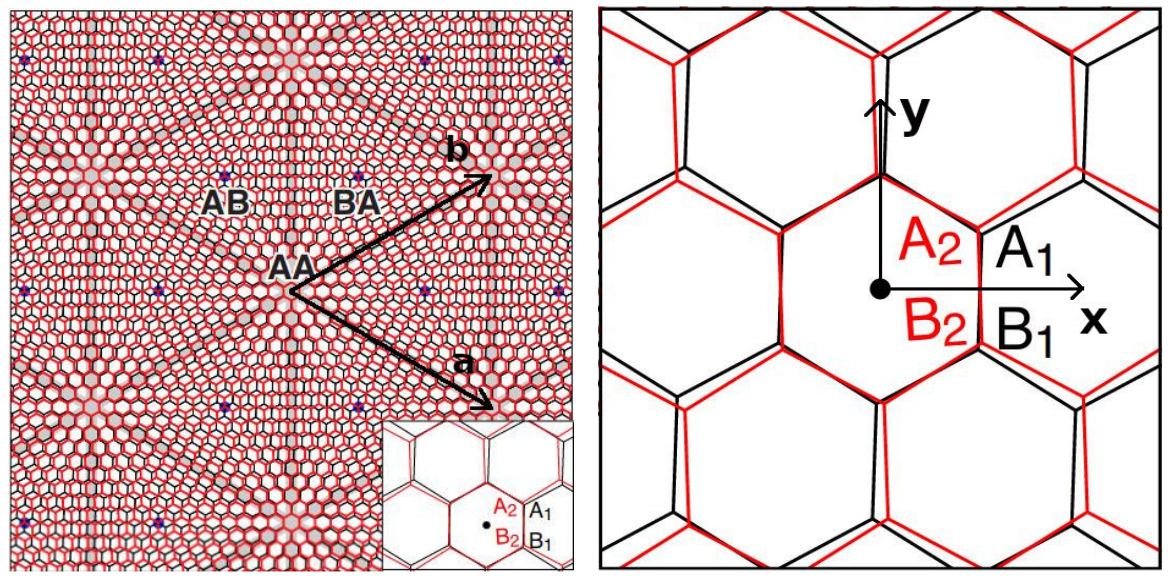
\includegraphics[height=.32\columnwidth]{fig/moireD6.png}
\caption{Commensurate $D_6$-type structure obtained by twisting the two layers from the initial AA stacking configuration, with the origin chosen as the center of the hexagons. Figure taken from \cite{thesis_rennella}.}
\label{fig:moireD6}
\end{figure}

\begin{figure}[H]
\centering
\begin{subfigure}{.5\textwidth}
  \centering
  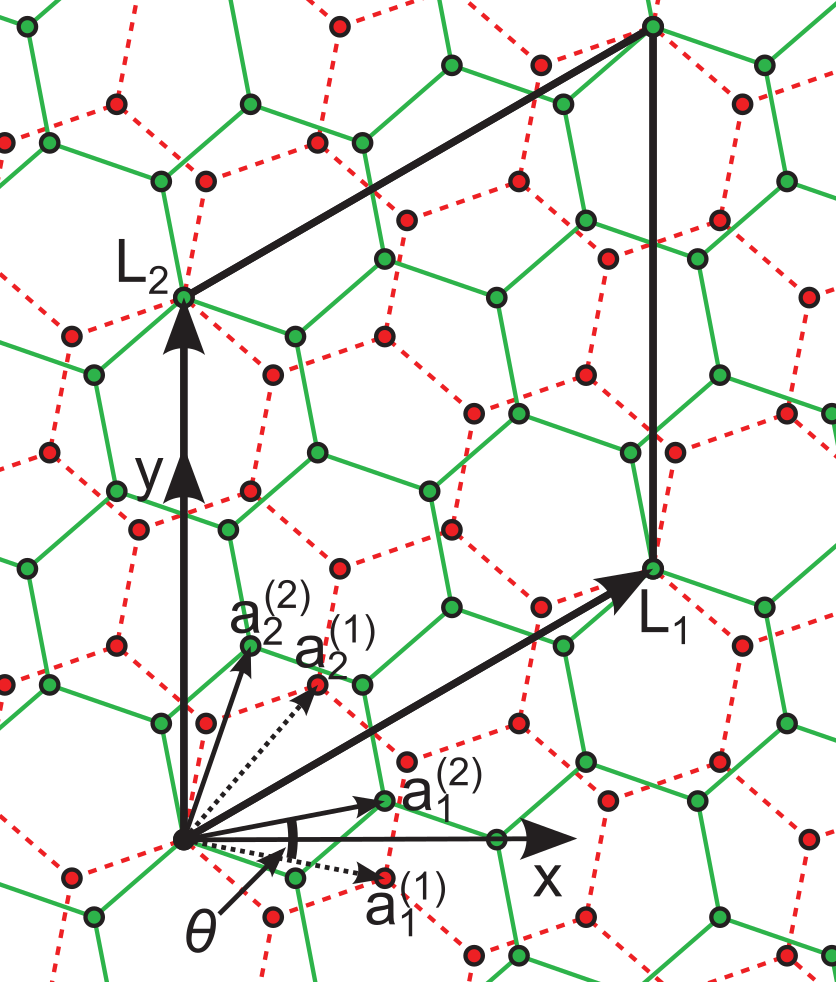
\includegraphics[height=.6\linewidth]{fig/latvec.png}
  \caption{}
  \label{fig:latvec}
\end{subfigure}%
\begin{subfigure}{.5\textwidth}
  \centering
  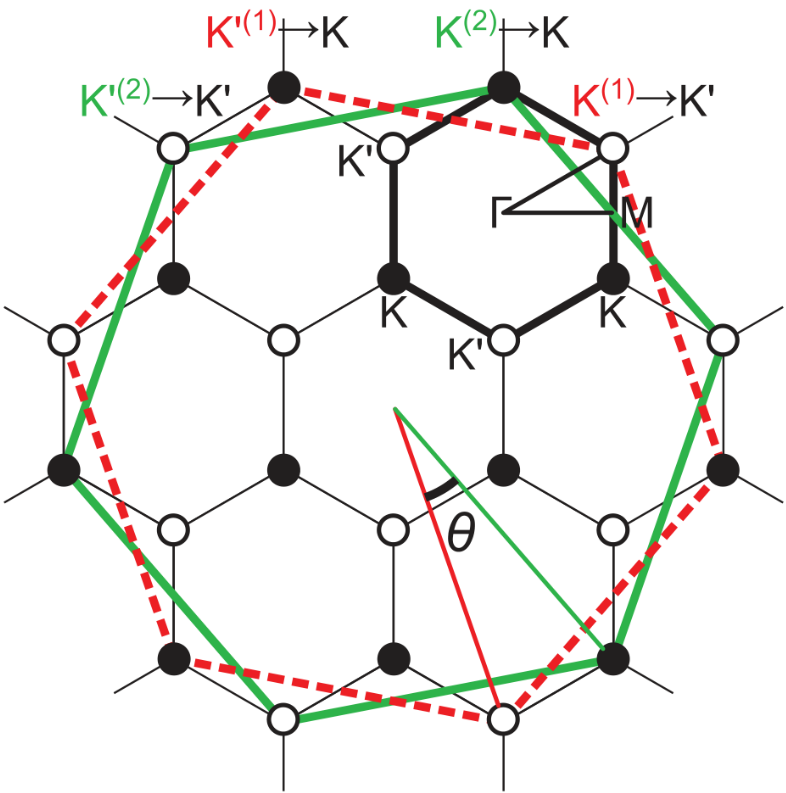
\includegraphics[height=.6\linewidth]{fig/bzminibz.png}
  \caption{}
  \label{fig:bzminibz}
\end{subfigure}
\caption{(a) Commensurate structure and lattice vectors $\vb{L}_1$, $\vb{L}_2$. (b) Monolayers (red and green) and mini BZ's with $(m,n) = (1,2)$ and $\theta = 21.8^\circ$. Figures taken from \cite{koshino2012}.}
\label{fig:geometry}
\end{figure}

%As drawn in Figure \ref{fig:latvec}, we have
%\begin{align}
%\label{eq:scalarprods1}
%\vb{a}_1^{(1)} \vdot \vb{a}_2^{(1)} &= a^2 \cos(60^\circ) = a^2/2; \\
%\label{eq:scalarprods2}
%\vb{a}_1^{(1)} \vdot \vb{a}_1^{(2)} &= a^2 \cos\theta; \\
%\label{eq:scalarprods3}
%\vb{a}_1^{(1)} \vdot \vb{a}_2^{(2)} &= a^2 \cos(60^\circ + \theta); \\
%\label{eq:scalarprods4}
%\vb{a}_1^{(2)} \vdot \vb{a}_2^{(1)} &= a^2 \cos(60^\circ - \theta).
%\end{align}

The superlattice vectors $\vb{L}_1$, $\vb{L}_2$ are related by a $60^\circ$ rotation. In general, because $\vb{L}_1$ belongs to the lattices of both layers, it can be parameterized by integers $m,n,m',n'$ as
\begin{equation} \label{eq:L1}
\vb{L}_1 = m\vb{a}_1^{(1)} + n\vb{a}_2^{(1)} = m'\vb{a}_1^{(2)} + n'\vb{a}_2^{(2)},
\end{equation}
where $\vb{a}_j^{(\ell)}$ is the $j$-th unit vector of layer $\ell$.

There is an appropriate choice of vectors $\vb{a}_i^{(\ell)}$ such that the indices $(m',n')$ are equal to $(n,m)$ \cite{koshino2012}. With this choice, one obtains the condition of commensurability
\begin{equation} \label{eq:costheta}
\cos\theta = \frac{m^2 + n^2 + 4mn}{2(m^2 + n^2 + mn)} = \frac{3 m^2 + 3mr + r^2/2}{3m^2 + 3mr + r^2},
\end{equation}
where $r = n-m$, and $\gcd(m,n) = \gcd(m,r)=1$. By taking the norm of $\vb{L}_1$ from Eq. \eqref{eq:L1} and using the angle relation in Eq. \eqref{eq:costheta}, the superlattice constant $L = \abs{\vb{L}_1} = \abs{\vb{L}_2}$ is given by
\begin{equation} \label{eq:commensurate-constant}
L(\theta) = a\sqrt{m^2 + n^2 + mn} = \frac{\abs{m-n}}{2 \sin(\theta/2)} \, a.
\end{equation}

The area of an unit cell of the superlattice is $A = \frac{\sqrt{3}}{2} L^2 = (m^2 + n^2 + mn) \, A_1$, where $A_1 = \frac{\sqrt{3}}{2} \, a^2$ is the area of unit cell of monolayer graphene. Considering the Brillouin Zone area (BZ), we have
\begin{equation} \label{eq:bz-volume}
\Omega = \frac{\Omega_1}{m^2 + n^2 + mn},
\end{equation}
where $\Omega_1 = (2\pi)^2/A$ is the monolayer's BZ area and $\Omega$ is the area of the moiré mini BZ. As an example, for $(m,n) = (1,2)$ we have $\theta = 21.8^\circ$ and $m^2 + n^2 + mn = 7$, therefore the monolayer BZ fits 7 mini BZ's in its area, as we see in Figure \ref{fig:bzminibz}.

\n

From the discussion above, one would conclude that a commensurate TBG system should have a translational symmetry with lattice constant $L(\theta)$ given by Eq. \eqref{eq:commensurate-constant}. However, as discussed in \cite{zou2018}, scanning tunneling microscopy (STM) experiments actually observe a moiré lattice constant
\begin{equation} \label{eq:STM-constant}
L'(\theta) = \frac{a}{2 \sin(\theta/2)} \leq L(\theta).
\end{equation}

This can be interpreted as MATBG exhibiting an approximate translational symmetry with superlattice constant $L'(\theta)$, despite optionally possessing an exact translational symmetry with $L(\theta)$ in the commensurate case. The Bistritzer-MacDonald (also known as continuum theory) to be derived in Section \ref{sec:BM-model} incorporates this translational symmetry and others ``good'' emergent symmetries that MATBG displays in experiments.


\subsection{Bistritzer-MacDonald model} \label{sec:BM-model}

The atoms positions of each layer are given by
\begin{equation} \label{eq:position-atoms-tbg}
\r = n_1 \a_{\ell,1} + n_2 \a_{\ell,2} + \vtau_{\ell,\alpha},
\end{equation}
where $\alpha = A,B$ indexes the site type, and $\tau_{\ell,\alpha}$ are basis vectors. The lattice vectors are the rotated $\a_{j}^{(\ell)} = R_{\theta_\ell} \a_{j}$, where
\begin{equation} \label{eq:rotation-matrix}
R_\theta =
\begin{pmatrix}
\cos\theta & -\sin\theta \\
\sin\theta & \cos\theta
\end{pmatrix},
\end{equation}
is the rotation matrix by an angle $\theta$ and we use the reference frame which $\theta_1 = -\theta/2$ and $\theta_2 = +\theta/2$. We shall consider AB-stacking as the starting position ($\theta=0$), because this is the most stable configuration for bilayer graphene \cite{handbook2019}. In this case, the translation vectors are given by
\begin{align}
\tau_{1,A} &= R_{-\theta/2}(0,0), \quad \tau_{2,A} = R_{\theta/2} [(0,-d) + \vtau_0], \label{eq:tauA} \\
\tau_{1,B} &= R_{-\theta/2}(0,d), \quad \tau_{2,B} = R_{\theta/2} [(0,0) + \vtau_0], \label{eq:tauB}
\end{align}
where $\vtau_0$ is an arbitrary translation. For example, $\vtau_0 = (0,0)$ corresponds to AB-stacking and $\vtau_0 = (0, d)$ corresponds to AA-stacking.

Defining the wave vectors $\vb{G}_{\ell,1} = \vb{b}_{\ell,1}$, $\vb{G}_{\ell,2} = \vb{b}_{\ell,2}$ and $\vb{G}_{\ell,3} = \vb{b}_{\ell,1} - \vb{b}_{\ell,2}$, the moiré pattern can be interpreted by an beat effect with periodicity $\vb{b}_k^{\text{m}} = \vb{G}_{1,k} - \vb{G}_{2,k}$, \cite{handbook2019}:
\begin{equation} \label{eq:moire-bvecs}
\vb{b}_1^{\text{m}} = \sqrt{3} \abs{\Delta \K} \qty( \frac{1}{2}, -\frac{\sqrt{3}}{2}), \quad
\vb{b}_2^{\text{m}} = \sqrt{3} \abs{\Delta \K} \qty( \frac{1}{2},  \frac{\sqrt{3}}{2}),
\end{equation}
where $\K$ is a Dirac point of an unrotated monolayer, and $\Delta\K = \K_1-\K_2$ with $\abs{\Delta \K} = 2 \abs{\K} \sin(\theta/2)$.

\n

The Hamiltonian $H$ of the model comes from a tight-binding approach $H = H_1 + H_2 + H_{\perp}$, where $H_\ell$ is the hamiltonian of the layer $\ell$, and $H_\perp = V_{12} + V_{12}^\d$ describes the interlayer hybridization. We write this hamiltonian in terms of Bloch waves
\begin{equation} \label{eq:BM-blochwave}
\ket{\psi_{\ell, \k, \alpha}} = \frac{1}{\sqrt{N_\ell}} \sum_{\R_\ell} e^{i \k \vdot (\R_\ell + \vtau_{\ell,\alpha})} \ket{\ell, R_\ell, \alpha},
\end{equation}
where $\ell$ labels the layer, $N_\ell$ is the number of unit cells, $\R_\ell$ are the positions of the underlying Bravais lattice, $\vtau_{\ell,\alpha}$ are the orbital centers (of sublattice $\alpha = A,B$) in the unit cell, and $\ket{\ell,\R_\ell,\alpha}$ are localized Wannier states. In this basis, considering only nearest-neighbor intralayer hopping, the low-energy hamiltonian of each layer is
\begin{equation} \label{eq:blg-eachlayer-hamil-lowenergy}
H^{\pm \K}(\q) = \hbar v_F \abs{\q}
\begin{pmatrix}
0 & e^{\mp i (\theta_\q - \theta_\ell)} \\
e^{\pm i (\theta_\q - \theta_\ell)} & 0
\end{pmatrix},
\end{equation}
where we expanded $\k = \pm \K_\ell + \q$ to first-order in $\q$.

\n

The interlayer Hamiltonian in second quantization reads
\begin{equation} \label{eq:interlayer-hopping}
V_{12} = \sum_{\R_1,\alpha,\R_2,\beta} c_{1,\alpha}^\d t_{12}^{\alpha\beta}(\R_1,\R_2) c_{2,\beta}(\R_2), \quad
t_{12}^{\alpha\beta}(\R_1,\R_2) =
\mel{1,\R_1,\alpha}{V_{12}}{2,\R_2,\beta}.
\end{equation}

Performing the Fourier transformation
\begin{equation} \label{eq:blg-fourier}
c_{\ell,\alpha}^\d(\R_\ell) = \frac{1}{\sqrt{N_\ell}} \sum_{\k_\ell}
e^{-i\k_\ell \vdot (\R_\ell + \vtau_{\ell,\alpha})} c_{\ell,\alpha}^\d(\k_\ell),
\end{equation}
with the sum of $\k_\ell$ over the BZ of layer $\ell$, we have
\begin{equation} \label{eq:interlayer-hopping-kspace}
V_{12} = \sum_{\k_1,\alpha,\k_2,\beta} c_{1,\alpha}^\d(\k_1) T_{12}^{\alpha\beta}(\k_1,\k_2) c_{2,\beta}(\k_2),
\end{equation}
\begin{equation} \label{eq:interlayer-hopping-Tkspace}
T_{12}^{\alpha\beta}(\k_1,\k_2) =
\frac{1}{\sqrt{N_1 N_2}} \sum_{\R_1,\R_2} e^{-i\k_1\vdot(\R_1+\vtau_{1,\alpha})}
t_{12}^{\alpha\beta}(\R_1,\R_2) e^{i\k_2\vdot(\R_2+\vtau_{2,\beta})}.
\end{equation}

Assuming the interlayer hopping $t_{12}^{\alpha\beta}(\R_1,\R_2)$ is only a function of the separation between the centers of the two orbitals, we can apply a Fourier transformation
\begin{equation} \label{eq:interlayer-hopping-fourier}
t_{12}^{\alpha\beta}(\R_1,\R_2) = t_{12}^{\alpha\beta}(\R_1+\vtau_{1,\alpha}-\R_2-\vtau_{2,\beta}) =
\int \frac{\dd[2]{\p}}{(2\pi)^2} e^{i \p \vdot (\R_1+\vtau_{1,\alpha}-\R_2-\vtau_{2,\beta})} t_{12}^{\alpha\beta}(\p).
\end{equation}

Plugging Eq. \eqref{eq:interlayer-hopping-fourier} in Eq. \eqref{eq:interlayer-hopping-Tkspace}, we obtain
\begin{equation} \label{eq:interlayer-hopping-simplified}
T_{12}^{\alpha\beta}(\k_1,\k_2) = \frac{1}{A_1}
\sum_{\G_1, \G_2} e^{i\G_1\vdot\vtau_{1,\alpha}} t_{12}^{\alpha\beta}(\p)
e^{-i\G_2\vdot\vtau_{2,\beta}} \delta_{\k_1+\G_1, \k_2+\G_2},
\end{equation}
where the crystal momentum coupling $\k_1 + \G_1 = \k_2 + \G_2$ is known as generalized umklapp condition.

\n

Equation \eqref{eq:interlayer-hopping-simplified} relies on the functional form of $t_{12}^{\alpha\beta}(\mathbf{p})$. In order to make further progress, we introduce additional assumptions. Given that both $A$ and $B$ sites of graphene correspond to a $p_z$ orbital of carbon atoms, we assume that $t_{12}^{\alpha\beta}(\r) = t_\perp(\r)$ does not depend on $\alpha$ or $\beta$. In \cite{tperp-laissardiere2012}, the authors characterize the behavior of $t_\perp(\r)$ using Slater-Koster parameters and numerically evaluate $t_\perp(\mathbf{p})$ through Eq. \eqref{eq:interlayer-hopping-fourier}. They establish that $t_\perp(\p)$ is solely a function of $\abs{\p}$ with rapid decay. This has significant implications, as only a few umklapp processes contribute to the coupling in Eq. \eqref{eq:interlayer-hopping-simplified}.

\n

In the small angle limit $\theta \lesssim 10^\circ$, we can expand $\k_\ell = \K_\ell + \q_\ell$ around the Dirac points of each layer, with $\abs{\q_\ell} \sim \abs{\Delta \K} \ll \abs{\K}$. Approximating $t_\perp(\K_1+\q_1+\G_1) \approx t_\perp(\K_1+\G_1)$, the interlayer coupling becomes
\begin{equation} \label{eq:interlayer-hopping-truncation}
T_{12}^{\alpha\beta}(\q_1,\q_2) = \frac{1}{A_{1}} \sum_{\G_1,\G_2} e^{i\G_1\vdot\vtau_{1,\alpha}}
t_{12}^{\alpha\beta}(\K_1+\G_1) e^{-i\G_2\vdot\vtau_{2,\beta}}
\delta_{\K_1+\q_1+\G_1,\K_2+\q_2+\G_2}.
\end{equation}

As $t_\perp(\p)$ rapidly decays with $\abs{\p}$, we truncate $t_\perp(\p) \approx 0$ for $\abs{\p} > \abs{\K}$. This leaves us with only three options for $\G_\ell$, where it can be either $\g_{\ell 1} = 0$, $\g_{\ell 2} = \b_{\ell 2}$, or $\g_{\ell 3} = -\b_{\ell 1}$. These options correspond to the three equivalent Dirac points on the monolayer Brillouin zone. Therefore, the crucial quantity becomes $t\perp(\abs{\K})$. This truncation leaves us with the term
\begin{equation} \label{eq:delta-term}
\delta_{\K_1+\q_1+\G_1,\K_2+\q_2+\G_2} = \delta_{\q_2-\q_1,\K_1-\K_2+\G_1-\G_2}.
\end{equation}

Since $\abs{\q_\ell} \ll \abs{\K}$, we find that the condition $\q_2-\q_1 = \K_1-\K_2+\G_1-\G_2$ is true only when $\G_1 = \g_{1n}$ and $\G_2 = \g_{2n}$ have the same index $n$. Consequently, we encounter three possibilities of momentum transfer:
\begin{equation} \label{eq:qb}
\q_\text{b} = \K_1 - \K_2 = \abs{\Delta \K} \, \qty(0, -1),
\end{equation}
\begin{equation} \label{eq:qtr}
\q_\text{tr} = (\K_1 - \K_2) + (\g_{12} - \g_{22}) = \abs{\Delta \K} \, \qty(\frac{\sqrt{3}}{2}, \frac{1}{2}),
\end{equation}
\begin{equation} \label{eq:qtl}
\q_\text{tl} = (\K_1 - \K_2) + (\g_{13} - \g_{23}) = \abs{\Delta \K} \, \qty(-\frac{\sqrt{3}}{2}, \frac{1}{2}),
\end{equation}

Finally, the interlayer coupling ends up with only three terms
\begin{equation} \label{eq:interlayer-3terms}
T_{12}^{\alpha\beta}(\q_1,\q_2) =
T^{\alpha\beta}_{\q_\text{b}} \delta_{\q_1-\q_2, \q_\text{b}} +
T^{\alpha\beta}_{\q_\text{tr}} \delta_{\q_1-\q_2, -\q_\text{tr}} +
T^{\alpha\beta}_{\q_\text{tl}} \delta_{\q_1-\q_2, -\q_\text{tl}},
\end{equation}
where
\begin{equation} \label{eq:interlayer-tensor}
T^{\alpha\beta}_{\q_n} = \frac{t_\perp(\abs{\K})}{A_{\text{u.c.}}} e^{i \g_{1n} \vdot \bm{\tau}_{1\alpha}}
e^{-i \g_{2n} \vdot \bm{\tau}_{2\beta}}.
\end{equation}

Writing matrices in the $A, B$ basis we get
\begin{equation} \label{eq:T-qb}
T_{\q_\text{b}} = \frac{t_\perp(\abs{\K})}{A_{\text{u.c.}}}
\begin{pmatrix}
1 & 1 \\
1 & 1
\end{pmatrix},
\end{equation}
\begin{equation} \label{eq:T-qtr}
T_{\q_\text{tr}} = \frac{t_\perp(\abs{\K})}{A_{\text{u.c.}}} e^{-i \g_{12} \vdot \vtau_0}
\begin{pmatrix}
e^{i\phi} & 1 \\
e^{-i\phi} & e^{i\phi}
\end{pmatrix},
\end{equation}
\begin{equation} \label{eq:T-qtl}
T_{\q_\text{tl}} = \frac{t_\perp(\abs{\K})}{A_{\text{u.c.}}} e^{-i \g_{13} \vdot \vtau_0}
\begin{pmatrix}
e^{-i\phi} & 1 \\
e^{i\phi} & e^{-i\phi}
\end{pmatrix},
\end{equation}
where $\phi = 2\pi/3$.


\subsection{Aspects of Group Theory applied to MATBG} \label{sec:grouptheory}

As discussed in \cite{zou2018}, at currently accessible energy scales, experiments indicate that MATBG exhibits some approximate symmetries. These include translational symmetry characterized by the constant $L' = a / (2 \sin\theta/2)$, valley symmetry $U_v(1)$, $C_{2z} \mathcal{T}$, and $D_6$ point group symmetry, which are not fully captured by a generic commensurate structure described in Section \ref{sec:tbg_geom}. The continuum model outlined in Section \ref{sec:BM-model} incorporates all these ``good'' symmetries. In this section, we will explore group theory concepts that will later be applied to understand the Wannier Obstruction \cite{zou2018} and the Topological Heavy Fermion model of MATBG \cite{topoheavyfermion2022}.

\subsubsection{Space groups} \label{sec:spacegroups}

The concept \textit{space group} refers to the spatial symmetries that preserve a crystal's structure. We denote an element of a space group $G$ as $\sg{R_\alpha}{\vtau}$, where $R_\alpha$ represents a point group operation such as rotations, reflections, inversions, or improper rotations, and $\vtau$ is a translation. A useful matrix representation for $G$ is:
\begin{equation} \label{eq:spacegroup-rep}
\sg{R_\alpha}{\vtau} =
\begin{pmatrix}
1 & 0 \\
\vtau & R_\alpha
\end{pmatrix},
\end{equation}
where $0$ is a row of three zeros, $\vtau$ is a column vector and $R_\alpha$ is $3\times 3$ rotation matrix.

In this representation, the product of two elements can be evaluated by multiplying the corresponding matrices:
\begin{align}
\begin{split}
\sg{R_\beta}{\vtau_2} \sg{R_\alpha}{\vtau_1} &=
\begin{pmatrix}
1 & 0 \\
\vtau_2 & R_\beta
\end{pmatrix}
\begin{pmatrix}
1 & 0 \\
\vtau_1 & R_\alpha
\end{pmatrix} \\
&= \begin{pmatrix}
1 & 0 \\
R_\beta \vtau_1 + \vtau_2 & R_\beta R_\alpha
\end{pmatrix}
= \sg{R_\beta R_\alpha}{R_\beta \vtau_1 + \vtau_2}.
\end{split}
\end{align}

The inverse of an element is given by
\begin{equation} \label{eq:inv-spacegroup}
\sg{R_\alpha}{\vtau}^{-1} =
\begin{pmatrix}
1 & 0 \\
-R_\alpha^{-1}\vtau & R_\alpha^{-1}
\end{pmatrix} =
\sg{R_\alpha^{-1}}{-R_\alpha^{-1}\vtau}.
\end{equation}

The pure translations and point group symmetries are the most evident, but a space group can also include compound operations, adding further complexity. The presence of these compound operations leads to the classification of space groups into \textit{symmorphic} or \textit{non-symmorphic}. We say that $G$ is symmorphic if, with a suitable choice of origin, all its elements can be decomposed in the form $\sg{R_\alpha}{\vtau} = \sg{1}{\R} \sg{R_\alpha}{0}$, where $\R$ is a Bravais lattice vector. In other words, $G$ is said to be symmorphic if it is a semi-direct product of the translation and point groups. For our purposes, the MATBG system exhibits emergent symmetries compatible with the $P622$ space group \cite{thesis_rennella}, which is symmorphic and associated with the $D_6$ point group.

\begin{table}[H]
\caption{Character table of point group $D_6$.}
\centering
\begin{tabular} { c c c c c c c  }
\specialrule{0.05em}{0em}{0.2em}
$\P$ & $\P E$ & $\P C_2$ & $\P2C_3$ & $\P2C_6$ & $\P3C_2'$ & $\P3C_2''$ \\
\specialrule{0.01em}{0.2em}{0.2em}
$A_1$ & $\P1$ & $\P1$ & $\P1$ & $\P1$ & $\P1$ & $\P1$ \\
\specialrule{0.01em}{0.2em}{0.2em}
$A_2$ & $\P1$ & $\P1$ & $\P1$ & $\P1$ & $ -1$ & $ -1$ \\
\specialrule{0.01em}{0.2em}{0.2em}
$B_1$ & $\P1$ & $ -1$ & $\P1$ & $ -1$ & $\P1$ & $ -1$ \\
\specialrule{0.01em}{0.2em}{0.2em}
$B_2$ & $\P1$ & $ -1$ & $\P1$ & $ -1$ & $ -1$ & $\P1$ \\
\specialrule{0.01em}{0.2em}{0.2em}
$E_1$ & $\P2$ & $ -2$ & $ -1$ & $\P1$ & $\P0$ & $\P0$ \\
\specialrule{0.01em}{0.2em}{0.2em}
$E_1$ & $\P2$ & $\P2$ & $ -1$ & $ -1$ & $\P0$ & $\P0$ \\
\specialrule{0.05em}{0.2em}{0em}
\end{tabular}
\label{tab:D6}
\end{table}

Although the continuum model incorporates the point group $D_6$, the regions of interest for localizing Wannier orbitals are the AB and BA regions of Figure \ref{fig:moireD6} as they are the most stable. These regions share certain symmetry properties, which can be described by the concept of \textit{Wyckoff position}, to be defined in the following section \ref{sec:wyckoff}. Once these concepts are understood, we can utilize the character table \ref{tab:D6} and its irreducible representations to construct Wannier orbitals centered at AB and BA regions.

\subsubsection{Site-symmetry group and Wyckoff positions} \label{sec:wyckoff}

Let $G$ be a space group associated with its corresponding lattice and choice of origin. The subgroup of all symmetry operations of $G$ that leave a point $P$ in real space invariant is called the \textit{site-symmetry group} of $P$. This point $P$ is called \textit{of special position} with respect to $G$ if there is at least one non-trivial (not the identity) symmetry operation of $G$ that leaves $P$ invariant.

For a general operation $g$ of $G$, the point $P$ will be mapped to some other point $Q = g P$. If $P$ is of special position with site-symmetry group $G_P$, then $Q$ will also be of special position, and its site-symmetry group $G_Q$ will be a conjugate group of $G_P$, namely $G_Q = g G_P g^{-1}$. In fact, we have:
\begin{equation} \label{eq:special-position}
G_Q Q = g G_P g^{-1} Q = g G_P P = g P = Q.
\end{equation}

When we apply all operations of $G$ to $P$, we obtain the \textit{crystallographic orbit} of $P$, which is the set of points $Q$ with site-symmetry groups conjugate to $G_P$. If $P$ is of special position, we call its crystallographic orbit a \textit{Wyckoff position} of the space group $G$. Therefore, the concept of a Wyckoff position refers to a set of points of special position with site-symmetry groups that are conjugates of each other.

\n

For TBG, we focus on the Wyckoff position $2c$, corresponding to the AB and BA regions of interest in Figure \ref{fig:moireD6}. The site-symmetry groups of these regions are all isomorphic to the point group $D_3$, a subgroup of $D_6$. In contrast, the $AA$ regions belong to Wyckoff position $1a$, and their site-symmetry groups have higher symmetry $D_6$.

Our next step will involve studying how to find the set of Wannier orbitals centered on the $2c$ Wyckoff position of the Moiré pattern and implementing a corresponding tight-binding model \cite{thesis_rennella}.

\section{DMFT Benchmark: The Hubbard model} \label{sec:hubbard}

Considering hopping only between nearest-neighbors, in second quantization the Hubbard Hamiltonian reads
\begin{equation} \label{eq:hubbard-hamiltonian}
H = \eps_d \sum_{i, \s} n_{i\s} +  \sum_{\nn{i}{j}, \s} t_{ij} (c_{i\s}^\d c_{j\s} + \hc)
+ U \sum_{i} n_{i\up} n_{i\down},
\end{equation}
where $\eps_d$ is the on-site energy, $t$ is the hopping amplitude, $U$ is represents the Coulomb repulsion, $c_{i\s}^\d$ ($c_{i\s}$) is the creation (annihilator) operator, and $n_{i\s} = c_{i\s}^\d c_{i\s}$.

The relatively simple Hamiltonian in Eq. \eqref{eq:hubbard-hamiltonian} exhibits a Metal-Insulator transition at half-filling ($n = \sum_{i\sigma} \ev{n_{i\sigma}} / N = 1$). To capture this transition, methods that account for electron correlations are essential. A powerful approach to achieve this is Dynamical Mean-Field Theory (DMFT) \cite{georges1996}, which provides a robust framework for studying real strongly correlated materials \cite{haule_real_materials}.

\subsection{Dynamical Mean-Field Theory (DMFT)} \label{sec:dmft}

The Dynamical Mean-Field Theory (DMFT) consists in a self-consistent mapping of the original Hamiltonian onto a local impurity model \cite{thesis_dmft_graz}. Its applicability stems from its exactness in the limit of infinite lattice coordination ($z \to \infty$) \cite{georges1996}. In this limit, the self-energy $\displaystyle{\lim_{z \to \infty}\Sigma(\mathbf{k},\omega) = \Sigma(\omega)}$ becomes independent of the momentum $\mathbf{k}$. This property proves itself very reliable in capturing the essential physics of strongly correlated systems.

In the context of the Hubbard model, the Hamiltonian is self-consistently mapped onto the Single Anderson Impurity Model (SIAM) \cite{impurity-solvers, georges1996}, where an interacting impurity, indexed by $d$, is coupled to a non-interacting external bath:
\begin{equation} \label{eq:anderson-hamiltonian}
H_{\text{SIAM}} = \underbrace{U n_{d\up} n_{d\down} + \eps_d \sum_{\s} n_{d\s}}_{H_{\text{imp}}}
+ \underbrace{\sum_{\k,\s} (t_\k c_{d\s}^\d c_{k\s} + \hc)}_{H_{\text{coup}}}
+ \underbrace{\sum_{\k,\s} \eps_\k c_{\k\s}^\d c_{\k\s}}_{H_{\text{bath}}}.
\end{equation}

In Eq. \eqref{eq:anderson-hamiltonian}, $H_{\text{bath}}$ is the Hamiltonian of the bath, $H_{\text{coup}}$ is the coupling between the bath and the single impurity $d$, and $H_{\text{imp}}$ is the hamiltonian of the impurity. The impurity Hamiltonian $H_{\text{imp}}$  has an interaction $U$ when two electrons are on the same site, anologous to the Hubbard Hamiltonian in Eq. \eqref{eq:hubbard-hamiltonian},.

There are several methods, known as impurity solvers, available in the literature which are designed to solve systems such as the SIAM. Reference \cite{impurity-solvers} gives an overview and a benchmark of some impurity solvers. By ``solving an impurity problem'', we actually mean determining the retarded Green's function of the impurity site $G_{\text{imp}}(\omega)$, because its knowledge allows us compute the spectral function $\displaystyle{\rho(\omega) = - \Im{G_{\text{imp}}(\omega)}} / \pi$ and a manifold of important observables related to transport \cite{pedagogical-gfs}.

Having in mind this auxiliary impurity problem, the DMFT scheme is based on the approximation
\begin{equation} \label{eq:dmft-approx}
\Sigma(\k, \omega) \approx \Sigma(\omega),
\end{equation}
where we assume that the self-energy is approximately independent of $\k$. Additionally, the self-consistency condition implies that the local lattice Green's function $G_{\text{loc}}(\omega)$ coincides with the impurity model's Green function $G_{\text{imp}}(\omega)$, and this fact translates into a convergence criterion for the DMFT algorithm.

Using Eq. \eqref{eq:dmft-approx}, the local Green's function in the continuum limit is
\begin{equation} \label{eq:Gf-local}
G_{\text{loc}}(\omega) = \sum_{\k} \frac{1}{\omega-\eps_\k-\Sigma(\k, \omega)} \approx
\int \dd{\eps} \frac{\rho_0(\eps)}{\omega - \eps - \Sigma(\omega)},
\end{equation}
where $\rho_0(\eps)$ is the non-interacting density of states (DOS) and depends only on the considered lattice structure.

In essence, the general DMFT algorithm works as follows. Firstly, we start with an initial guess for the self-energy $\Sigma(\omega)$ and compute $G_{\text{loc}}(\omega)$ by Eq. \eqref{eq:Gf-local}. Next, the impurity solver takes as input the bath hybridization function
\begin{equation} \label{eq:hybridization-func}
\Delta(\omega) = \omega - \eps_d - G_{\text{loc}}^{-1}(\omega) - \Sigma(\omega),
\end{equation}
and computes $G_{\text{imp}}(\omega)$. Next, $G_{\text{loc}}$ and $G_{\text{imp}}$ are compared with some convergence criterion and, if not satisfied, we update the self-energy by Eq. \eqref{eq:self-energy-update} and come back to the beginning of the loop.
\begin{equation} \label{eq:self-energy-update}
\Sigma(\omega) = \omega - \eps_d - G_{\text{imp}}^{-1}(\omega)
\end{equation}

Finally, the filling $n$ is given by \cite{bruus}
\begin{equation} \label{eq:filling}
n = \int_{-\infty}^{\infty} f(\omega, T) \rho(\omega) \dd{\omega},
\end{equation}
where $f(\omega, T) = (e^{\omega/k_B T} + 1)^{-1}$ is the Fermi-Dirac distribution at temperature $T$.

\subsection{Bethe lattice} \label{sec:bethe}

The Bethe lattice is an infinite lattice where each site has $z$ neighbors and any two sites are connected by a unique shortest path. In our work, we focused on the special case of the Bethe lattice with infinite coordination $z\to\infty$, because DMFT is exact and its algorithm simplifies in this setting. The Hubbard Hamiltonian in Eq. \eqref{eq:hubbard-hamiltonian} only makes sense with $z\to\infty$ if the hopping amplitude is renormalized as \cite{thesis_bruno}
\begin{equation} \label{eq:hopping-renormalization}
t = \frac{t_*}{\sqrt{z}},
\end{equation}
where $t_*$ is the renormalized hopping, which we used $2t^* = 1$ as our energy unit.

For the Bethe lattice, one can obtain the simplified relation \cite{thesis_bruno}
\begin{equation} \label{eq:simple-hybridization-bethe}
\Delta(\omega) = t_*^2 \, G_{\text{imp}}(\omega),
\end{equation}
which simplifies the loop, since $\Delta(\omega)$ can be directly inserted in the impurity solver.

\subsection{Impurity Solver} \label{sec:impurity-solver}

As our main objective was to establish a working code for DMFT, we chose to use the Non-Crossing Approximation (NCA) impurity solver. As shown in Table 1 of \cite{impurity-solvers}, the NCA has a low computational cost while still providing reasonable qualitative results. However, as discussed in \cite{vildosola2015}, it is important to note that it does not return accurate quantitative estimates for the critical interaction values $U_{c1}$, $U_{c2}$, and for the Kondo temperature $T_{\text{K}}$ \cite{haule_real_materials, vildosola2015}. The NCA method also has the advantage of quickly accessing a versatile range of temperatures. The details of the NCA can be found in Section 2.2 of \cite{thesis_bruno}. For our work, we used the code developed by Kristjan Haule, which is publicly available at \cite{hauleweb}.


\subsection{Results} \label{sec:results}
% \ALERT{$\eps_d \to \eps_d/U$, Figure \ref{fig:UxT-rho0}(e-f)}

We explored how the system behaves when one deviates from particle-hole symmetry (PHS), where $\eps_d = U/2$. When the temperature is sufficiently low, the system undergoes a phase transition at two distinct values of $U$. Starting from a Mott insulating solution at large $U$ and gradually decreasing it, the system reaches a critical value $U_{c_1}$, at which it becomes metallic. Conversely, starting from a metallic state at low $U$ and increasing it, the system reaches another critical value $U_{c2} > U_{c1}$, at which it transitions back to an insulator. To characterize these two phases, we use the spectral density at zero energy \cite{georges1996} and the filling $n$, as half-filling is a necessary condition for the insulating phase.

Figure \ref{fig:UxT-rho0} is a color plot of $\rho(0) = (\rho_{\text{metal}}(0) + \rho_{\text{insul}}(0))/2$ as a function of $U \times T$, where the ``metal'' and ``insul'' labels mean starting with a metallic (low $U$) or insulating (high $U$) solution. The blue region (where $\rho(0) = 0$) corresponds to the insulating phase and the red region (where $\rho(0)$ is maximum) to the metallic phase. The green region is a coexistence phase, where $\rho(0)$ changes abruptally to an intermediate value. The critical point $(U_c, T_c)$ identify the vertice of the coexistence region (``green triangle'').

%\begin{center}
%\ALERT{NAS FIGURAS DO Uc e Tc DEVERIA SER O XLABEL $\eps_d/U$.}
%\end{center}

\begin{figure}[H]
\centering
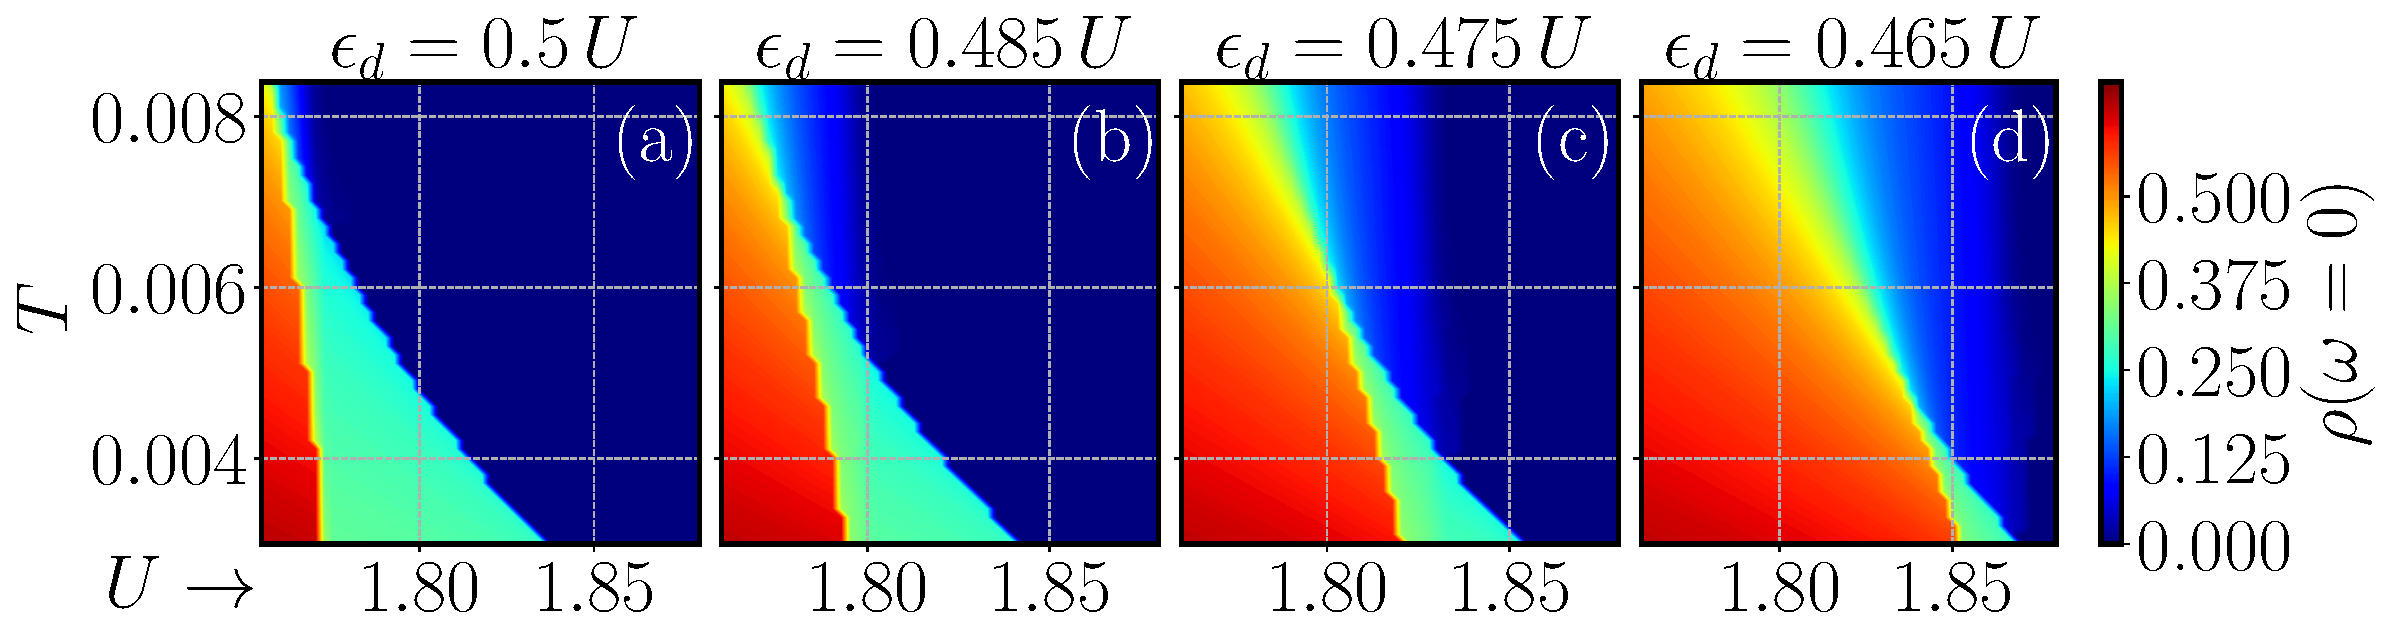
\includegraphics[width=0.8\columnwidth]{fig/fig2-abcd-eps-converted-to.pdf}
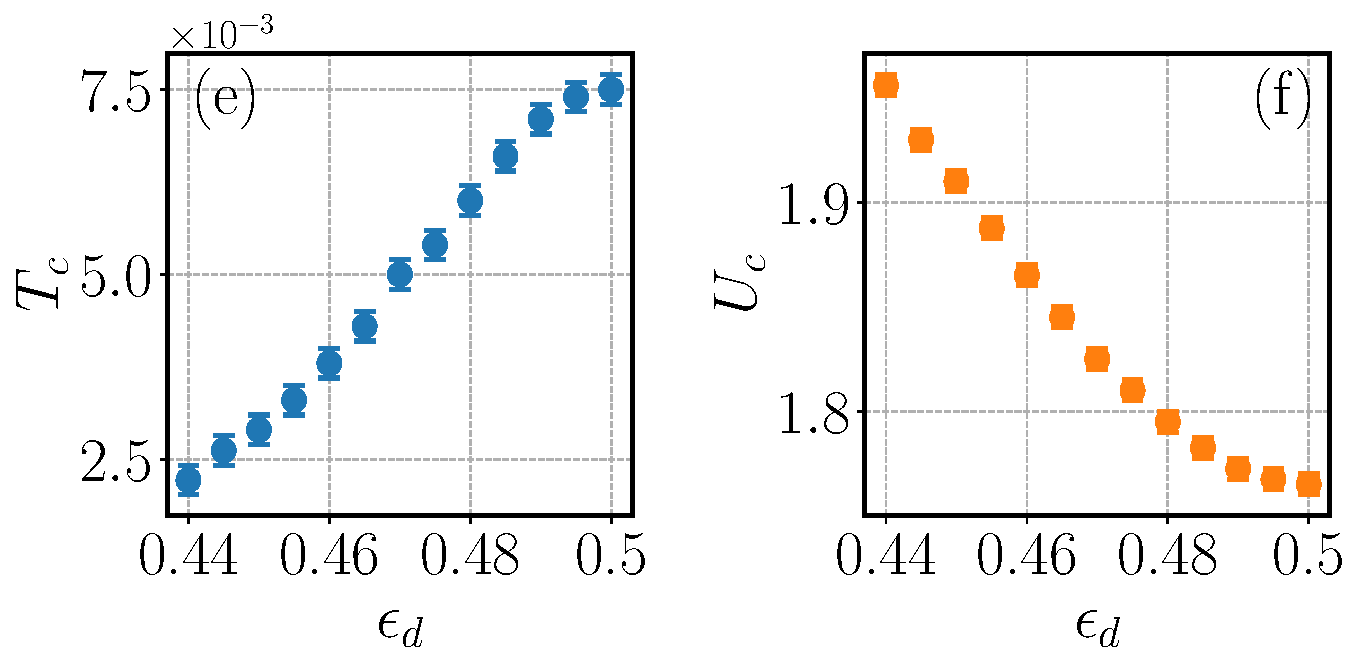
\includegraphics[width=0.48\columnwidth]{fig/fig2-ef-eps-converted-to.pdf}
\caption{(a-d) Phase diagrams $U \times T$ as $\eps_d$ is moved away from $U/2$. (a) $\epsilon_d=0.5U$ (b) $\epsilon_d=0.485U$ (c) $\epsilon_d=0.475U$ (d) $\epsilon_d=0.465U$. (e-f) $U_c, T_c$ as functions of $\eps_d/U$. }
\label{fig:UxT-rho0}
\end{figure}

Figure \ref{fig:T0002-butterfly} shows $U \times \eps_d$ phase diagrams for the fixed temperature $T = 0.002$, where $\Delta \rho(0) = \rho_{\text{metal}}(0) - \rho_{\text{insul}}(0)$, $n = (n_{\text{metal}} + n_{\text{insul}})/2$, $\Delta n = n_{\text{metal}} - n_{\text{insul}}$. The ``smile pattern'' of Figures \ref{fig:T0002-butterfly}(a,b,d) identifies the coexistence region.

\begin{figure}[H]
\centering
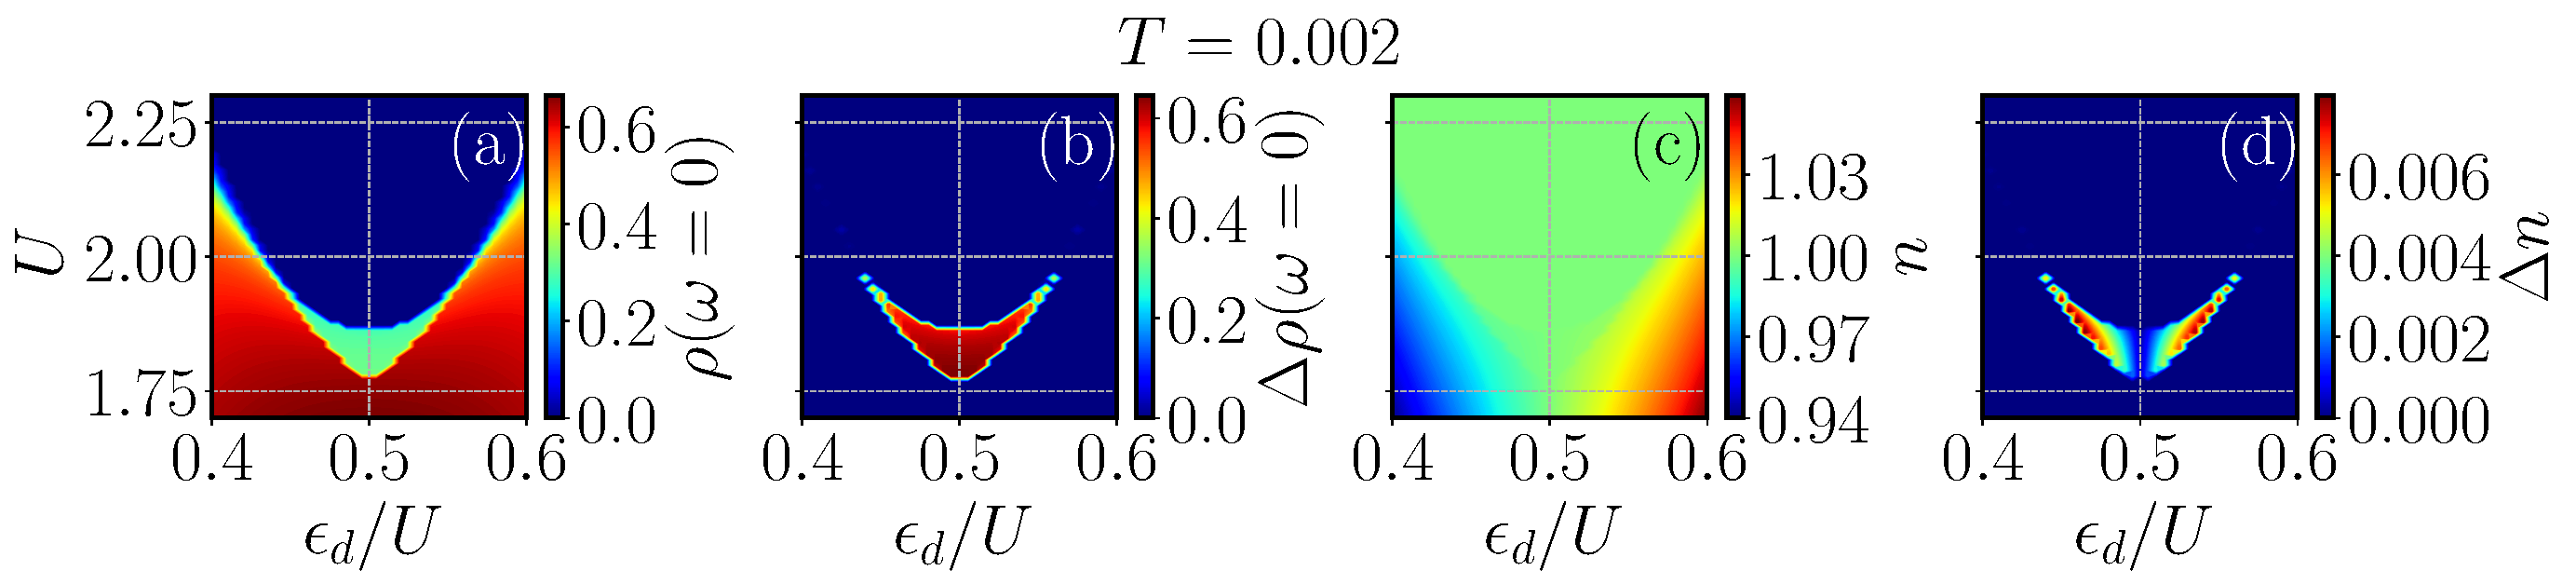
\includegraphics[width=\columnwidth]{fig/fig4-abcd-eps-converted-to.pdf}
\caption{Phase diagrams $U \times \epsilon_d$ for $T=0.002$. (a,b) average $(\text{M}+\text{I})/2$ and difference $(\text{M}-\text{I})$ for $\rho(\omega=0)$. (c,d) average and difference for the filling $n$. }
\label{fig:T0002-butterfly}
\end{figure}




\pagebreak


\chapter{Evaluation of the Institutional Support received during the period} \label{chp:apoioInst}
%\chapter{Description and evaluation of the Institutional Support received during the period} \label{chp:apoioInst}

During the period covered by this report, the student used the Research Overhead to acquire the Acer Nitro 5 AN515-58-58W3 laptop, which was extensively used for the heavy DMFT calculations in Section \ref{sec:results}.


\chapter{Participation in scientific events} \label{chp:particEvento}

The student participated in the following scientific events/courses:

\begin{itemize}
\item Attended as a listener the \href{https://www.ictp-saifr.org/apsmarch23/}{APS/ICTP-SAIFR Satellite March Meeting} held on March 20-22, 2023, at ICTP-SAIFR.
\item Attended as a listener the \href{https://www.ictp-saifr.org/qm2023/}{Workshop on Strong Electron Correlations in Quantum Materials: Inhomogeneities, Frustration, and Topology} held on June 19-23, 2023, at ICTP-SAIFR.
\item Participated in Luis Gregório G. V. Dias da Silva's research group Journal Club during 2023 and 2024 at USP.
\item Presented the results from Section \ref{sec:results} in a poster entitled ``Charge density signatures of the Mott transition in the particle-hole asymmetric Hubbard model at finite temperatures'' at the \href{https://www1.fisica.org.br/~eosbf/2024/index.php/en/}{2024 Autumn Meeting of the Brazilian Physical Society} held on May 19-23, 2024, at UFSC, Florianópolis - SC.
\end{itemize}


\chapter{Conclusions and Future Activities} \label{chp:conclusions}

In Section \ref{sec:tbg}, we presented our research on TBG theory. We derived the Bistritzer-MacDonald model \cite{macdonald2011} in Section \ref{sec:BM-model}. Our intention is to utilize this knowledge to develop our own code for analyzing the electronic properties of the system. The BM model is advantageous as it is independent of whether a configuration of TBG is commensurate or not, and it also incorporates all the emergent symmetries observed in experiments \cite{zou2018}. In order to construct the Wannier orbitals localized on the AB and BA regions of interest, we recognized the necessity of thoroughly reviewing concepts of group theory in Section \ref{sec:grouptheory}. Our studies will enable us to employ group theory to elucidate the Wannier Obstruction \cite{zou2018} and the Topological Heavy Fermion model \cite{topoheavyfermion2022}.

In Section \ref{sec:hubbard}, we established a fully operational DMFT algorithm and extensively explored the phase diagrams for the Metal-Insulator transition. In Figure \ref{fig:UxT-rho0}(a), we successfully replicated a known result from the literature for $\eps_d = U/2$ \cite{georges1996}. Additionally, we conducted a thorough investigation of the asymmetric case, which has received comparatively less attention in the literature. Notably, we analyzed the expansion of the coexistence region as we deviated from the particle-hole symmetric (PHS) case and observed the distinctive ``smile'' pattern in the $U \times \eps_d$ phase diagrams of Figure \ref{fig:T0002-butterfly}. Looking ahead to our DMFT progress, our goal is to enhance and extend the algorithm for the study of TBG. However, before developing a practical implementation, we acknowledge the necessity of comprehensively understanding the intrinsic properties of the system through a rigorous analysis of its symmetries.

%%-----
%% Referências bibliográficas
%%-----
\addcontentsline{toc}{chapter}{\bibname}
%\bibliographystyle{abntex2-num}
\bibliography{bibliografia}
\bibliographystyle{ieeetr}


%%-----
%% Fim do documento
%%-----

\end{document}
